% 
%% \documentclass[paper=a4,fontsize=12pt,open=right,noabbrev]{report}
% \documentclass[12pt]{report}
% \usepackage[utf8]{inputenc}
% \usepackage{amsmath}
% \usepackage{amssymb}
% \usepackage{graphicx}
% \usepackage{placeins}
% \usepackage{cite}
% \usepackage{physics} 
% \usepackage{mathrsfs} 
% \usepackage{geometry}  
% \usepackage{layouts} 
% \usepackage{newfloat}
% \usepackage{float}
% 
% \setlength{\parindent}{0em}
% \setlength{\parskip}{1em}
% 
% 
% % Technical point floatstyle
% \floatstyle{ruled}
% \newfloat{Technical Point}{htbp}{lop}[chapter]
% 
% 
% \begin{document}



\chapter{Complementary Aspects}
\label{ch:Complementary}
The described method was developed and constructed to reweight dynamical data in form of Markov State Models (MSM) between non-equilibrium steady states (NESS). The procedure in its current form is based on ideas from stochastic thermodynamics, coarse-graining of trajectories by MSMs and the Maximum Caliber. We want to discuss in this chapter how these ideas can be expanded in other applications than reweighting simulated data.

The defined ensembles and the parallels to equilibrium statistical mechanics raise the question if we can push this analogy further. In particular we will discuss if there is an invariant measure similar to the density of states (see section~\ref{sec:DoS}) that depends on the interaction of the system but not on thermodynamic variables. Other questions raised are the role of partition functions and the relation to thermodynamic variables based on derivatives. These relations in connection to the Maximum Caliber were discussed by Dill et al.~\cite{dixit2018perspective} for trajectory ensembles under global constraints.  Equilibrium statistical ensembles were also expanded to quantum mechanical systems. In combination with the discrete nature of MSMs, it can be beneficial to analyse such systems in the context of the presented ensembles. The laser system in section~\ref{sec:Lasersys} is such an example. It was approximated classically because simulation of quantum mechanical systems is beyond the scope of this thesis. 

The definition of the NESS ensembles is based on local entropy productions between discretised states. We will examine how this discretisation of dynamics is related to the underlying continuous trajectories. This will open up another way of estimating local entropy productions by trajectory averaging over an ensemble of single trajectories.

%At last we can discuss the construction of NESS-MSMs. Equilibrium MSMs can be constructed by inferring detailed balance on the data to converge MSM with less data available~\cite{bowman2009progress}. A similar approach can be applied here: Local entropy production and global balance were shown to be fundamental information on NESS ensembles. Enforcing them on a NESS would increase efficiency of MSM construction by inferring physical constraints.

\section{Invariant Quantity}
\label{sec:InvariantC}
An invariant has the property of not changing under a set of transformations. The density of states is one example under change of the Boltzmann measure (see section~\ref{sec:rewEqu}). It is defined by the number of microscopic states depending on chosen variables like energy and possibly other variables (see section~\ref{sec:DoS}). Once we have shown that systems are recovered under a certain transformation, we expect an underlying invariant measure. For the set of transformations used here, the \textit{dynamical invariant} was identified in section~\ref{sec:Invariant} by
\begin{equation}
    I_{ij}^2 = q_{ij} q_{ji} \exp \left ( \frac{c_i + c_j}{2}+ \zeta \right ) 
\end{equation}
and is presented for the minimal 1D system (see section~\ref{sec:1Dmodel}) in figure~\ref{fig:invariant}. Knowing the invariant of a system, one can construct any ensemble in NESS that we are interested in. The reweighting formula becomes
\begin{equation}
 p_{ij} = I_{ij} \exp \left ( \frac{1}{2} ( \tilde \zeta + \Delta S_{ij} )+ \frac{1}{4} (\tilde c_i + \tilde c_j)\right ),
\end{equation}
where $\mathbf{\tilde c}$ is determined by enforcing $\sum_k p_{ik}=1$ and applying the numerical solver used for the reweighting formula (see section~\ref{sec:numerics}). We want to understand the physical meaning of this quantity and show the technical use of it in enhanced sampling methods. 

\begin{figure}
 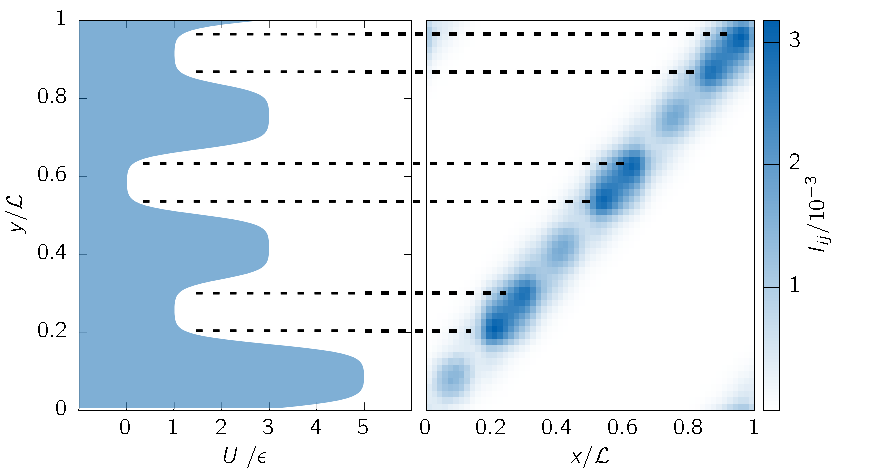
\includegraphics{../plots/Complementary/Invariant_2010.pdf}
 \caption[The dynamical invariant of the 1D driven system.]{The invariant of the 1D system. The potential surface is presented to indicate the positions of the maxima.}
 \label{fig:invariant}
\end{figure}

At first intuition the dynamical invariant is the density or number of trajectories connecting two microstates within lagtime $\tau$, equivalent to the density of states. However, this quantity is difficult to grasp because time and  length of trajectories have unknown relation without further information. We need thermodynamic properties like the diffusion coefficient $D = T\mu$, defined by the Einstein relation via temperature $T$ multiplied with the mobility $\mu$. For an ensemble of free diffusive single particles starting at position $X=0$ and time $t_0=0$ with diffusion coefficient $D$, the probability distribution at time $t$ is given by the solution to the Fokker-Planck equation~\cite{van1992stochastic}:
\begin{equation}
 P(X,t) = \frac{1}{\sqrt{4 \pi D t}} \exp \left (- \frac{X^2}{4Dt} \right ).
\end{equation}
The probability distribution is interpretable as the density of trajectories of length $t$ in free diffusion. The assumption  still holds for an invariant of NESS because a generalised diffusion coefficient was shown to depend on an effective temperature~\cite{lander2011mobility}. In any case, the invariant of the test 1D system in NESS in figure~\ref{fig:invariant} does not agree with the expected invariant. In fact it shows marks that originate from the potential and peak on top of the potential barrier and on the sides of the potential wells. The middle region of the potential wells show a lower invariant than its sides. This shows that the invariant depends on the temperature as expected but also on the potential surface. We believe that this dependence originates from the approximation used by the reweighting. A free diffusion invariant is expected for the full solution. An invariant for the full solution can be calculated if a numerical solution to the reweighting formula is found.


Nevertheless, the approximated invariant holds some information. We note from the definition that the matrix is symmetric. All information about dissipative effects are given by the local entropy productions.  The invariant on the other hand contains information about symmetric local fluctuations, or non-dissipative effect. These contributions were distinguished by Maes~\cite{maes2018non} showing that symmetric and asymmetric contributions to the dynamics are decoupled in equilibrium and coupled in off-equilibrium. The symmetric or \textit{frenetic} contribution can be defined by $A_{ij} = \sqrt{p_{ij}p_{ji}}$ such that $p_{ij}= A_{ij} \exp \left( \Delta S_{ij} /2 \right )$. The frenetic contribution changes with driving as predicted by Maes. The reweighting method uses information on dissipative dynamics but recovers these frenetic contributions correctly. We conclude that the invariant contains the necessary symmetric information. Accordingly we interpret the invariant as the non-dissipative local fluctuations of the system. 

This point of view explains why the reweighting scheme does not apply to temperature-reweighting. The chosen constraints infer information about  dissipative effects. The changes in the system under variation of temperature are in the non-dissipative part of the dynamics so it lies outside the scope of the presented method. It requires a different set of constraints that is unknown to us. 

The invariant is not completely understood, but it can be of computational purpose since it can be sampled from different simulations. This is the underlying idea of equilibrium enhanced sampling methods like multicanonical simulation \cite{janke1998multicanonical}, replica exchange \cite{sugita1999replica} or metadynamics\cite{laio2002escaping}. The general idea is to tweak the system such that regions of interest are sampled more frequently. This can be done by increasing the temperature to sample high-energy states more frequently or adding artificial potentials to push or attract the system in a certain direction. The changes do not have to be of physical nature and are removed from the system after taking advantage of better sampling conditions. All gathered information is collected in the invariant as long as the corresponding relations are known from a reweighting formula. These relations are for example based on the Boltzmann factor for the equilibrium ensembles or, here, the given reweighting relations for NESS.  The reweighting procedure can be combined with such sampling methods. This is a step to reach experimentally important timescales that are inaccessible by the limitation of computational power~\cite{perilla2015molecular}.

\section{Trajectory Analysis}
\label{sec:Trajectory}
MSMs are a coarse view on the dynamics of a system. The reweighting procedure acts on the MSM by enforcing the local entropy productions. We want to analyse how the single trajectories relate to the local entropy productions. The trajectory space allows us a detailed view on the system and one can judge if the microstate of the MSM and the assumptions for the analytic solution (see section~\ref{sec:Sprod}) are chosen correctly. The analytic solution ignores effects of fluctuations on the entropy production, the trajectory analysis takes them into account. Furthermore, the analytic solution for the entropy production only works when the new forces are applied along the collective variables (CV) chosen for the MSM. A trajectory analysis allows us to calculate entropy productions for forces depending on other system variables.
\begin{figure}
\centering
 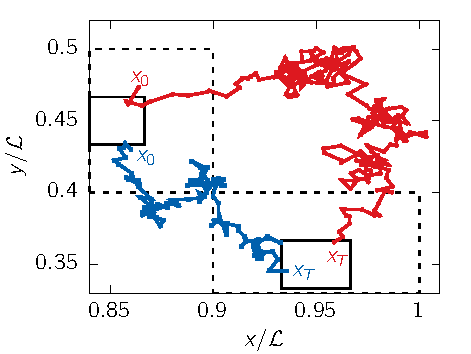
\includegraphics{../plots/Complementary/traj.pdf}
 \caption[Two example trajectories from simulation of the 2D system between two microstates.]{Two example trajectories from simulation of the 2D system between two microstates. The dashed boxes show the microstates, the solid boxes show the core of the microstates. A trajectory is counted when it starts and finishes in a core-state. }
 \label{fig:traj}
\end{figure}

MSMs are sampled by counting all trajectories that start in a given microstate $i$ and finish in another microstate $j$. The transition probabilities are defined by a trajectory ensemble average (see section~\ref{sec:StochTherm}) connecting two microstates
\begin{equation}
 \langle \chi_i (\mathbf{x}_0) \chi_j(\mathbf{x}_T) \rangle = \int \int \dd{\mathbf{x}_0} \dd{[\mathbf{x}(t)]} p [\mathbf{x}(t) | \mathbf{x}_0] p(\mathbf{x}_0) \chi_i(\mathbf{x}_0) \chi_j(\mathbf{x}_T) ,
\end{equation}
where $\chi_i(\mathbf{x})$ is $1$ if $\mathbf{x}$ is in state $i$ and $0$ else, $\mathbf{x}_0$ is the initial point of the trajectory~$\mathbf{x}(t)$ and $\mathbf{x}_T$ the final point. Similarly we  use this to calculate the local entropy production from trajectory space
\begin{equation}
\begin{aligned}
  \langle \Delta S \rangle_{ij} &=  \langle \chi_i (\mathbf{x}_0) \chi_j(\mathbf{x}_T) \rangle \\ &= \int \int \dd{\mathbf{x}_0} \dd{[\mathbf{x}(t)]} p [\mathbf{x}(t) | \mathbf{x}_0] p(\mathbf{x}_0) \chi_i(\mathbf{x}_0) \chi_j(\mathbf{x}_T) \Delta S[\mathbf{x}(t)] ,
\end{aligned}
\end{equation}
where $\Delta S[\mathbf{x}(t)]$ is the entropy production of a trajectory that is calculated by 
\begin{equation}
\begin{aligned}
  \Delta S [\mathbf{x}(t)] \approx \frac{1}{2T} \sum_d \sum_{t=1}^{t=T} \left ( x^{(d)}_t - x^{(d)}_{t-1} \right ) \left ( F^{(d)}({\mathbf{x}}_t) + F^{(d)}({\mathbf{x}}_{t-1}) \right )
\end{aligned}
\end{equation}
in discrete form, discussed in section~\ref{sec:Sprod}. The relevant trajectories are chosen  as illustrated in figure~\ref{fig:traj}. The dashed lines represent a microstate, the box in the middle is the core state. A trajectory starts in a core state and terminates when the final core state is reached. The center state ensures that fluctuations on the boundaries are not taken into account.  A maximum length of trajectory is set for computational efficiency.
\begin{figure}[t]
\centering
 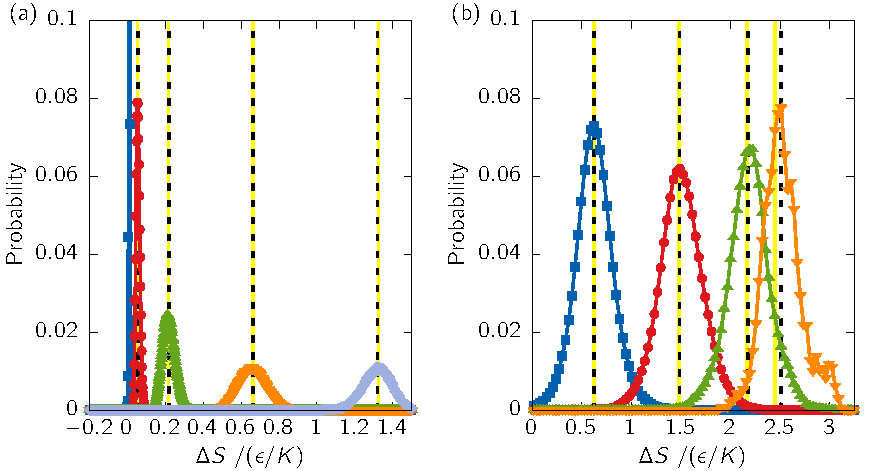
\includegraphics{../plots/Complementary/Shist.pdf}
 \caption[Distribution of entropy productions for the single particle in 1D potential and single particle in 2D potential for chosen transitions. ]{Distribution of entropy productions for (a) the single particle in 1D potential and (b) single particle in 2D potential for chosen transitions. The average of the distribution is shown by a black dashed line, the analytic solution is shown by a solid yellow line. }
 \label{fig:Shist}
\end{figure}
This does not influence the distributions of the entropy productions, shown for chosen transitions on the 1D and 2D model in figure~\ref{fig:Shist}.  The average of the distribution is shown by the dashed black line, the solid yellow line represents the average as calculated from the analytic model. The two values agree well, indicating that the analytic approximation works well on the coarse-grained level. Larger distances reduce the number of available trajectories and produce more noise. The full difference of analytic and measured value is shown in figure~\ref{fig:Sdiff} for the 1D system and locally for the 2D system.  We consider the trajectory analysis to be exact, because it takes all information into account and is sufficiently sampled for the given systems. The absolute deviations are small compared to the absolute entropy productions in the range $[-10\,\frac{\epsilon}{K},10\,\frac{\epsilon}{K}]$. Yet the 1D systems shows a pattern: When a trajectory start or ends in a state dominated by large local forces the deviation of the analytic solution is larger but still in an acceptable range. The deviation might originate from a non-symmetric distribution of entropy productions. This indicates that the fluctuations do not cancel each other out and the analytic assumption is flawed.  

A third way to estimate the entropy production is to use the transition probabilities of  the MSM by $ \ln \Delta S_{ij} = \frac{p_{ij}}{p_{ji}}$. This method agrees with the others but suffers from sampling issues for larger distances and needs longer simulation times to gather sufficient data, so it is not of further interest. The analytic method gives a good estimate and can thus be used for estimation of entropy productions without additional data used. The trajectory method can estimate the entropy production well but samples the whole distribution. It gathers more information than needed for the reweighting and requires simulation of the target system.  

The trajectory analysis is useful when one wants to reweight along forces not described by the CVs of the MSM.  The analytic method can only be used when the forces are defined on the same CV. Otherwise sampling the trajectories of the target system is the only way to estimate the target system for reweighting. One can sample the system at different thermodynamic states and gather the information at any of these states afterwards. Continuous reweighting is not possible in this case. The second use is testing for double peaks in the distribution of entropy productions. It indicates that two microstates are connected by more than one set of pathways. The MSM should be changed to resolve these pathways by a different choice of microstates. Otherwise the MSM is not able to distinguish all pathways and it would cause errors in the reweighting procedure. 
%The third use of the trajectory analysis is the efficient construction of MSM and is discussed in the next section

\begin{figure}[t]
\centering
 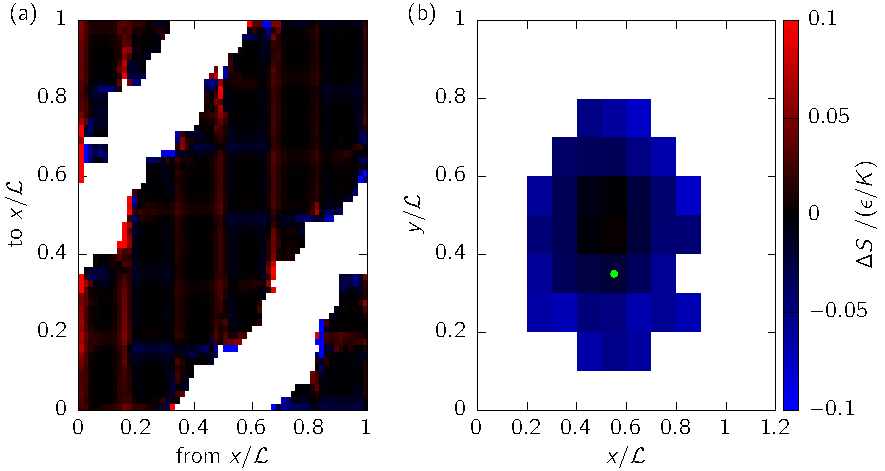
\includegraphics{../plots/Complementary/Sdiff.pdf}
 \caption[Deviation of local entropy production between analytic solution and averaging over simulated trajectories for (a) a single particle on a 1D potential surface and (b) a single particle on a 2D potential surface for a chosen starting point.]{Deviation of local entropy production between analytic solution and averaging over simulated trajectories for (a) a single particle on a 1D potential surface and (b) a single particle on a 2D potential surface for a starting point at (0.55,0.35), marked by the green dot.  }
 \label{fig:Sdiff}
\end{figure}


\section{Off-Equilibrium Reweighting in Literature}
Reweighting of dynamical data in and out of equilibrium has attracted some attention lately. Previous works were focused on reweighting dynamical ensembles of equilibrium systems, for instance using a Maximum Likelihood approach~\cite{chodera2011dynamical} or a Maximum Caliber approach~\cite{wan2016maximum}. It was shown how information can be drawn from non-equilibrium ensembles and combined at equilibrium~\cite{wu2016multiensemble}.  Here, we focus on the three works focussing on the problem for reweighting off-equilibrium dynamics. We want to discuss the assumptions of these methods and  compare them to our presented method. 

Two methods relying on the  Girsanov transformation~\cite{donati2017girsanov,warren2018trajectory} reweight each trajectory in conformational coordinates from the reference data individually. 
The first work by Warren and Allen relies on long trajectories and is tested successfully on a birth-death process in NESS. The authors point out two practical problems of the method: First they note that long trajectories are needed for unbiased reweighting and the length is set by the unknown target system. Second, the distribution of trajectory weights becomes broader with increasing trajectory length. These problems of long trajectories were avoided by Donati and Keller by employing short trajectories with Markov State Models. The method requires full data of the trajectories in conformational space and the random numbers generated during the simulation for the Langevin thermostat. Storing all this information would require large computational effort. In practice the lagtime of the MSM and the target state is defined before running the reference simulation and the trajectories are reweighted on runtime. It is  shown that the equilibrium MSM of a hexapeptide can be recovered. The method is combined with metadynamics~\cite{donati2018Girsanov} for efficient sampling of dynamics and construction of MSM. The reweighting method is in theory applicable for off-equilibrium MSMs, albeit it was not shown yet. In contrast, our method relying on the Maximum Caliber is applied a posteriori on an MSM. The target system can be chosen freely after the simulation data is gathered. The two methods mentioned above rely on reweighting every trajectory individually, forcing them to reweight during simulation runtime. Furthermore our method requires minimal computational effort by only solving a set of non-linear convex equations. The problem of long trajectories discussed by Warren and Allen was addressed by Markov State Modeling for both, the method of Donati and Keller and our method. 

Another new reweighting method applicable for NESS by Zuckermann et al.~\cite{russo2020iterative} was published by submission of this thesis. A number of short Markov-like trajectories are collected from a reference simulation. The target system for reweighting is defined by its stationary distribution. The weights of the reference trajectories are updated individually until they recover the target probability distribution and are stationary.  This algorithm can be extended to NESS by adding wells and sinks of probability at chosen positions. In this case the trajectories have to be arranged such that the probability is transported from well to sink while meeting the requirements on the stationary distribution. We refer to the paper for details of the algorithm. The method uses space discretisation like our method but does not require Markovianity unlike our method and the Girsanov reweighting. The trajectories are treated in their continuous form, similar to the Girsanov reweighting. This method was not yet tested on NESS systems.

The sparse number of works on reweighting dynamics off-equilibrium shows that it is a  new problem.  Most of the methods are only expected to work in off-equilibrium but are not tested yet. The presented methods rely on different theoretical bases and assumptions and operate on different spaces (long or short trajectories, MSM). We hope to see continuous work on this problem in the future.

%  to construct an MSM at equilibrium. It has been shown to be effiecient for a number of 


% \section{Markov State Model Construction}
% \label{sec:MSMCon}
% 
% 
% \bibliography{/home/marius/PhD/Thesis/references.bib}
% \bibliographystyle{plain}
% \end{document}
